\documentclass{article}
\usepackage{graphicx} % Required for inserting images
\usepackage[a4paper, left=3cm, right=2cm, top=2cm, bottom=2cm]{geometry}
\usepackage{float}
\usepackage{subcaption}  % For subfigure support
\usepackage{subfigure}


\title{Lab4 Report}
\author{Nguyen Thanh Tung - 2440047}
\begin{document}
\maketitle

\section{Labwork}

\begin{figure}[h!]
    \centering
    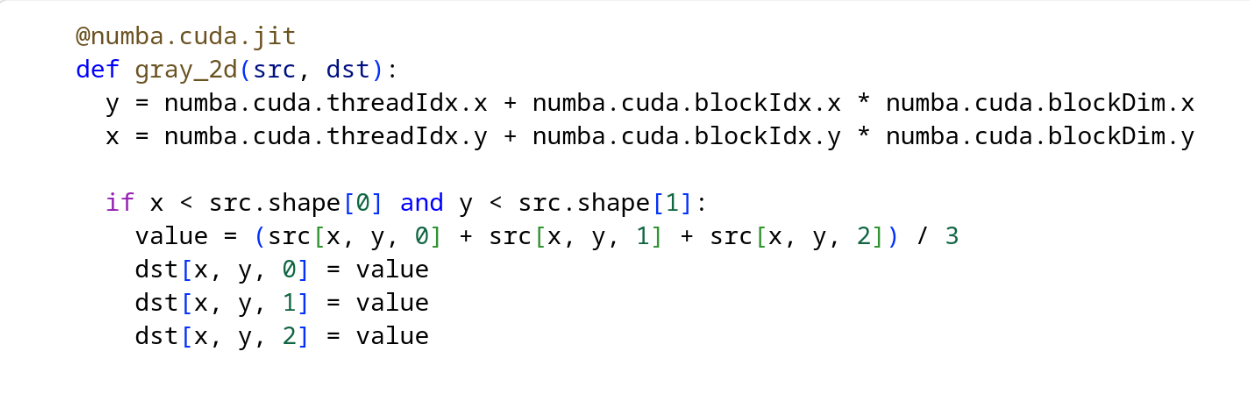
\includegraphics[width=1\linewidth]{impl.png}
    \caption{Kernel implementation}
    \label{fig:kernel}
\end{figure}


We implemented the kernel as shown in Figure \ref{fig:kernel}. We swap the block x and y dimensions with the image x and y dimensions to maximize the coalesced read and write. With that, we got 25\% speed up compared to 1d kernel (Figure \ref{fig:run}.

\begin{figure}[h!]
    \centering
    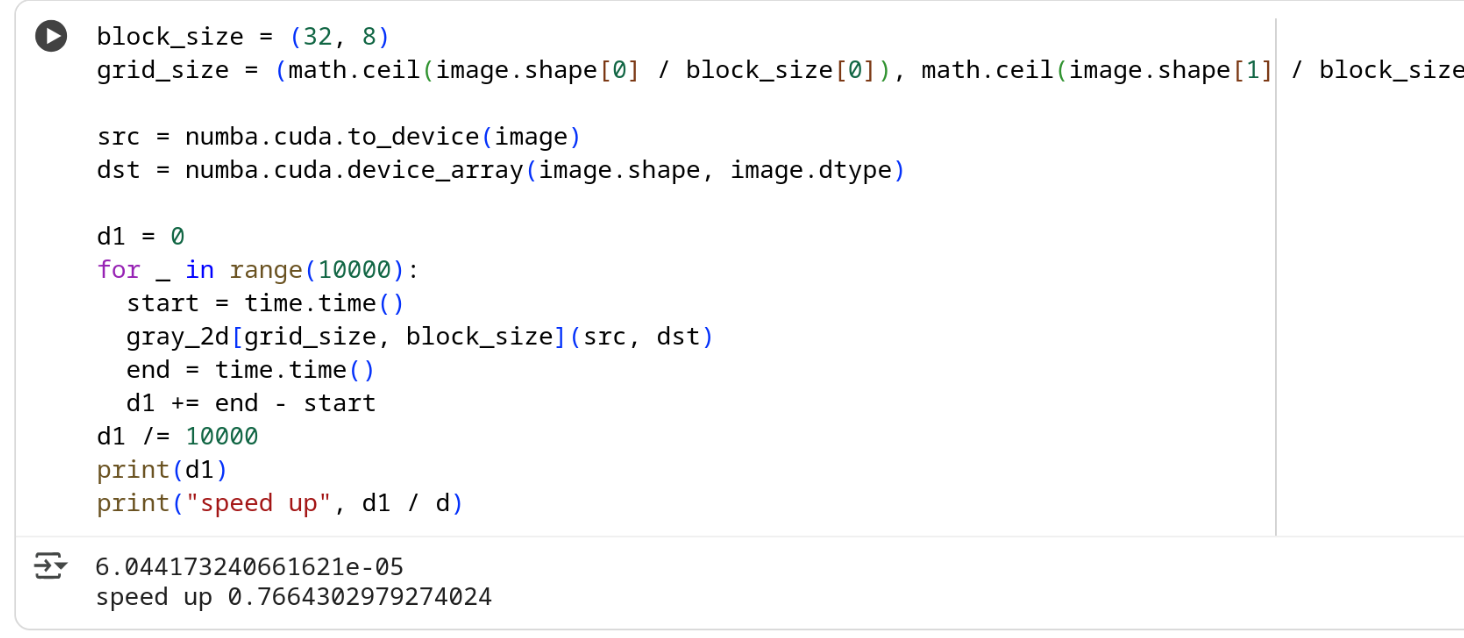
\includegraphics[width=0.5\linewidth]{run.png}
    \caption{2D kernel execution}
    \label{fig:run}
\end{figure}

The Figure \ref{fig:block-size} shows that the execution time decreases when we increase the block size.

\begin{figure}[h!]
    \centering
    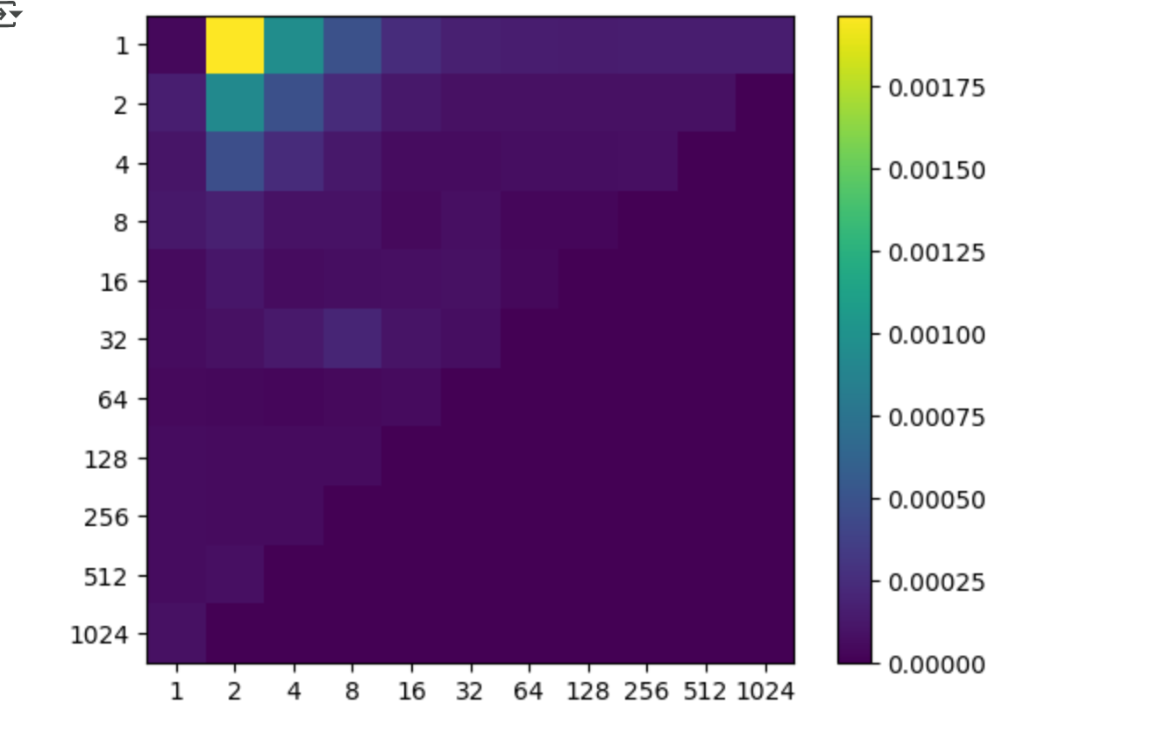
\includegraphics[width=0.5\linewidth]{block_size.png}
    \caption{Block size}
    \label{fig:block-size}
\end{figure}


\section{Exercise 1}
16x16 block is the best configuration with total of 16*16*4=1024 threads. The 8x8 block only get total 8*8*8=512 threads. The 32x32 is larger then the 512 threads per block.

\section{Exercise 2}
512 threads per block give the highest total threads: 512 * 3 = 1536 threads. The 128 threads per blocks result in 128 * 4 = 512 threads. the 256 threads per block result in 256 * 4 = 1024 threads. the 1024 threads per block result in 1024 * 1 = 1024 threads.

\section{Exercise 3}
The total number of block is ciel(2000 / 512) = 4.


\end{document}
